\documentclass{boi2014-lt}

\usepackage{enumitem}
\usepackage{wrapfig}
\usepackage{mathtools}
\usepackage{tikz}

\renewcommand{\DayNum}{1}
\renewcommand{\TaskCode}{coprobber}
\renewcommand{\TaskName}{Policininkas ir plėšikas}

\renewcommand{\labelitemii}{$\circ$}
\newcommand{\constant}[1]{{\tt #1}}

\begin{document}
    \begin{wrapfigure}[8]{r}{6cm}
        \vspace{-24pt}
		\includegraphics[width=6cm]{\TaskCode.jpeg}
	\end{wrapfigure}

	Bitangoje nusikalstamumo lygis muša visų laikų rekordus. Be kitų
	nusikaltimų, kasdien vyksta apiplėšimai. Kaskart įvykus nusikaltimui,
	siaurais skersgatviais, kurie jungia įvairius miesto užkampius, sprunkantį
	plėšiką tenka gaudyti vienišam policininkui. Deja, dažniausiai plėšikai
	pasprunka nuo persekiotojų, kadangi jie miestą pažįsta žymiai geriau už
	pareigūnus.

	Bitangos miesto policijos departamentas (BMPD) organizuoja aukščiausio
	lygio susitikimą dėl nusikalstamumo mažinimo. Viena jų iniciatyvų yra
	persekioti plėšikus į pagalbą pasitelkiant kompiuterį. Tam BMPD sudarė
	tikslų miesto žemėlapį. Dabar jiems reikia programinės įrangos, kuri
	sukurtų persekiojimo strategijas.

	Vieno pareigūno persekiojančio vieną plėšiką uždavinys modeliuojamas taip:
	\begin{enumerate}
		\item Policijos pareigūnas pasirenka vieną užkampį ir ima jame
			patruliuoti.
		\item Tada plėšikas pasirenka užkampį apiplėšimui (jis žino, kur yra
			pareigūnas). Daroma prielaida, jog nuo šios akimirkos ir
			pareigūnas, ir plėšikas žino vienas kito buvimo vietą.
		\item Policijos pareigūno ėjimo metu jis nukeliauja į gretimą užkampį
			(t.~y. užkampį, kurį su dabartiniu užkampiu jungia skersgatvis)
			arba laukia (t.~y. nepajuda niekur).
		\item Plėšiko ėjimo metu jis nukeliauja į gretimą užkampį. Atkreipkite
			dėmesį, jog priešingai negu policininkas, plėšikas laukti negali.
			Instinktas jiems liepia nepaliaujamai bėgti.
		\item Policijos pareigūnas ir plėšikas vienas po kito atlieka ėjimus
			(pirmas eina pareigūnas) kol kuri nors iš šių sąlygų tampa patenkinta:
			\begin{enumerate}
				\item situacija pasikartoja (situacija yra apibrėžta abiejų
					dalyvių pozicijomis bei kieno eilė yra daryti ėjimą).
					Tai reiškia, jog plėšikas sugebės išvengti policijos
					kiek norima ilgai, taigi plėšikas pasprunka;
				\item policijos pareigūnas ir plėšikas susitinka tame pačiame
					užkampyje po bet kurio iš jų ėjimo. Šiuo atveju policijos
					pareigūnas pagauna plėšiką.
			\end{enumerate}
	\end{enumerate}

    \Task
	Turite parašyti programą, kuri pagal duotą miesto žemėlapį nustatytų,
	ar įmanoma pagauti plėšiką, ir jeigu tai yra įmanoma, pagautų jį
	darydama ėjimus už policijos pareigūną.

	Jūsų programa turi daryti prielaidą, jog plėšikas juda optimaliai.

    \Implementation
    Turite realizuoti dvi funkcijas:
    \begin{itemize}
        \item \method{start(N, A)}, kuri priima šiuos argumentus:
            \begin{itemize}
                \item $N$ -- užkampių skaičius (užkampiai yra sunumeruoti
                    nuo $0$ iki $N-1$);
                \item $A$ -- dvimatis masyvas, apibūdinantis skersgatvius:
                    kiekvienam $0 \le i, j \le N-1$,
                    $$
                        A[i, j] \text{ is }
                        \begin{dcases*}
                            \texttt{false} & jeigu $i$ ir $j$ nejungia skersgatvis
                                \\
                            \texttt{true} & jeigu $i$ ir $j$ jungia skersgatvis
                        \end{dcases*}
                    $$
                    Visi skersgatviai bus dvikrypčiai (t.~y. $A[i, j] = A[j, i]$
                    su kiekviena galima $i$ ir $j$ reikšme) ir nebus jokių skersgatvių,
					jungiančių užkampį su juo pačiu (t.~y. $A[i, i]$ bus
                    \texttt{false} kiekvienam galimam $i$). Be to, galite daryti
					prielaidą, jog judant skersgatviais visada bus įmanoma iš bet kurio
					užkampio pasieki bet kurį kitą.
            \end{itemize}

		Jeigu duotame žemėlapyje įmanoma pagauti plėšiką, funkcija \method{start}
		turi grąžinti numerį užkampio, kuriame policijos pareigūnas pasirenka
		patruliuoti. Priešingu atveju, ji turi gražinti $-1$.

		\item \method{nextMove(R)}, kurios argumentas $R$ yra numeris užkampio,
			kuriame dabar yra plėšikas, ir turi grąžinti numerį užkampio,
			kuriame policijos pareigūnas bus po savo ėjimo.
    \end{itemize}

    Funkcija \method{start} bus iškviesta lygiai kartą, prieš bet kurį
    funkcijos \method{nextMove} iškvietimą. Jeigu \method{start} grąžina
    $-1$, tada \method{nextMove} nebus iškviesta. Priešingu atveju,
	\method{nextMove} bus pakartotinai kviečiama tol, kol baigsis
	persekiojimas.
    Tiksliau, programa baigs darbą atsiradus kuriai nors iš šių sąlygų:
    \begin{itemize}
        \item \method{nextMove} grąžina neleistiną ėjimą;
        \item situacija pasikartoja;
        \item plėšikas pagaunamas.
    \end{itemize}

    \Example
    \begin{wrapfigure}[4]{r}{2cm}
        \vspace{-0.5cm}
        \centering
        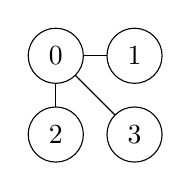
\begin{tikzpicture}
        \draw (0,1) -- (0,0);
        \draw (0,1) -- (1,0);
        \draw (0,1) -- (1,1);
        \foreach \x in {0,1} \foreach \y in {0,1}
            \draw (\x,\y) node[circle,draw,fill=white,inner sep=0,minimum size=0.7cm] {\pgfmathparse{int(2-2*\y+\x)}\pgfmathresult};
        \end{tikzpicture}
    \end{wrapfigure}
	Pažiūrėkime į dešinėje pavaizduotą pavyzdį. Šiuo atveju, bet kuris užkampis
	policijos pareigūnui yra gera pradinė pozicija. Jeigu jis pradės užkampyje
	Nr. 0, jis gali laukti savo pirmą ėjimą ir plėšikas pats pas jį atbėgs.
	Kitu atveju, jei jis pradės kuriame nors kitame užkampyje, jis gali laukti,
	kol plėšikas atsidurs užkampyje Nr. 0, ir tada nueiti į jį.
    
    Funkcijų vykdymo eiga galėtų būti tokia:

    \begin{tabular}{|l|c|}
        \hline
            {\bf Funkcijos kvietimas} & {\bf Grąžina} \\
        \hline
            \method{start(4, [[0, 1, 1, 1], [1, 0, 0, 0], [1, 0, 0, 0], [1, 0, 0, 0]])} &
            \constant{3} \\
        \hline
            \method{nextMove(1)} & \constant{3} \\
        \hline
            \method{nextMove(0)} & \constant{0} \\
        \hline
    \end{tabular}

	Pastaba: \method{start} kvietime trumpumo vardan \constant{false} žymima
	\constant{0} ir \constant{true} žymima \constant{1}.

\end{document}
